\documentclass[compress, aspectratio=169]{beamer}

%presentation layout

\mode<presentation>
{
  \usetheme{Berlin}
  % \usecolortheme{dove}
  \setbeamercolor{structure}{bg=white,fg=black}
  \setbeamercolor{normal text}{bg=white,fg=black}
  \setbeamercolor{titlepage}{bg=white,fg=black}
  \setbeamercolor{titlelike}{bg=white,fg=black}
  \setbeamercolor{palette primary}{bg=white}
  \setbeamercolor{palette secondary}{bg=gray, fg=white}
  \setbeamercolor{palette tertiary}{bg=gray, fg=white}
  \setbeamercolor{palette quarternary}{bg=white}
  \setbeamercovered{transparent}
  \useinnertheme{rectangles}
  %\usefonttheme{serif}
}

\setbeamertemplate{navigation symbols}{}

%loading packages
\usepackage[ngerman]{babel}
\usepackage[T1]{fontenc}
\usepackage[utf8]{inputenc}
\usepackage{graphicx}
\usepackage{amsmath}
\usepackage{framed}
\usepackage{caption}
\usepackage{subcaption}
\usepackage{multicol}

% vorgeplaenkel
\title[StAPf-Bericht]{StAPF-Bericht}

\author{Ständiger Ausschuss aller Physikfachschaften}

\institute[Zusammenkunft aller Physikfachschaften]

\date{20. Mai 2020}

\subject{Bericht des StAPF}

\begin{document}

\begin{frame}[plain]{}
  \titlepage
\end{frame}


\section{StAPF}

\begin{frame}
\centering
\Huge Berichte der ZaPF-Gremien
\end{frame}


\begin{frame}{Gewählte Mitglieder im StAPF}
\begin{minipage}{.5\textwidth}
\centering
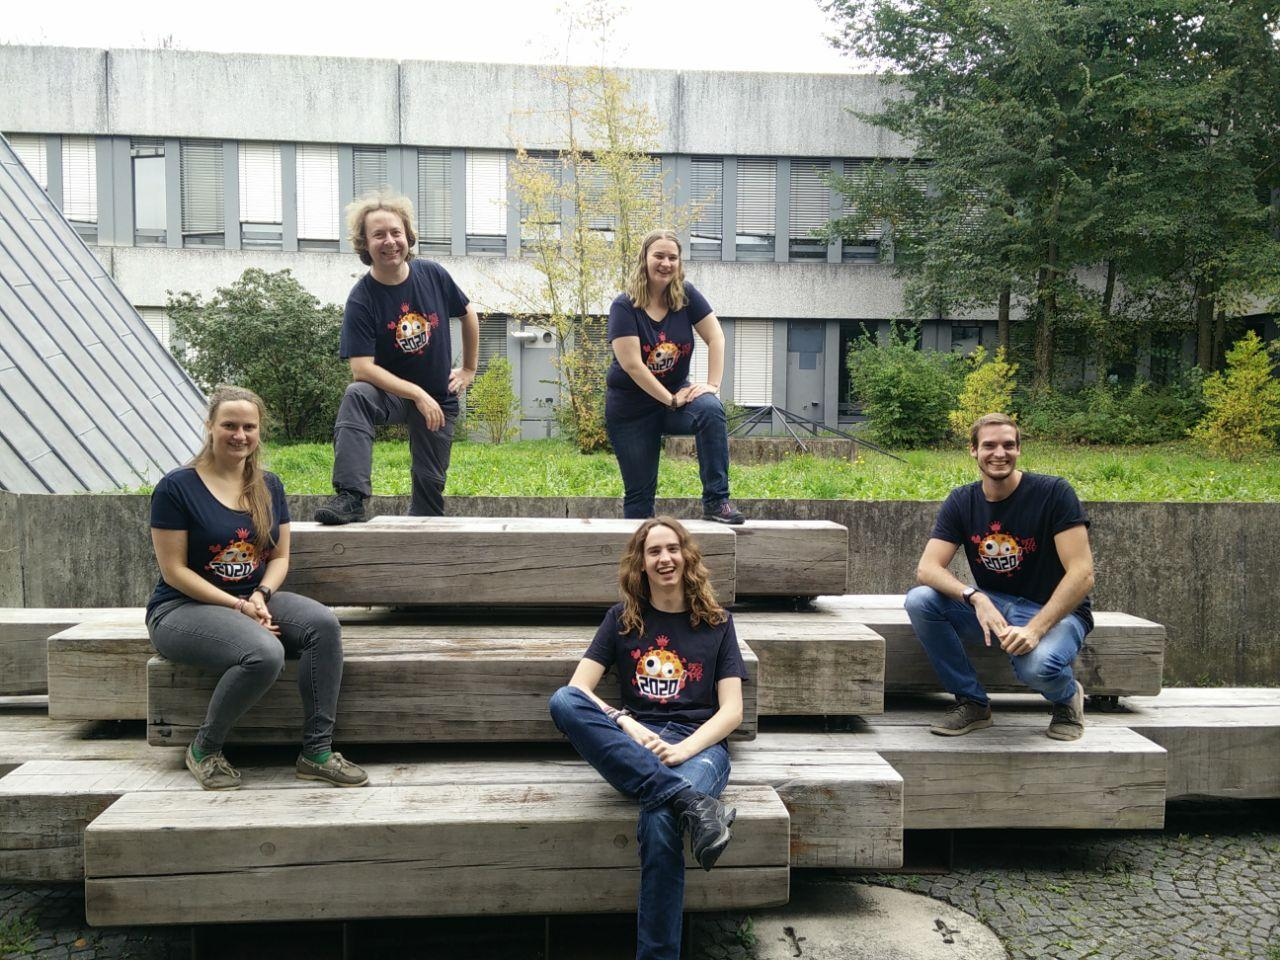
\includegraphics[width=.9\textwidth]{StAPF.jpg}
\vspace{.5cm}
\end{minipage}
\begin{minipage}{.45\textwidth}
Von links nach rechts:\\

Anna Summers (Uni Kiel)\\

Leon Nutzinger (FU Berlin)\\

Andreas Drotloff (Uni Würzburg)\\

Victoria Schemenz (Uni Potsdam)\\

Christoph Blattgerste (Uni Heidelberg)\\
\end{minipage}
\end{frame}

%\begin{frame}{Was bisher geschah...}
%  \begin{itemize}
%    \item Offener Brief zum Hochchulgesetz NRW versandt und beworben
%    \item Resolutionen verschickt und veröffentlicht
%    \begin{itemize}
%        \item Resolution zu Semesterzeiten \\
%          (mit KaWuM, BuFaTa ET, Komet, GeoDACH, BuFaK WiSo, PsyFaKo)
%        \item Resolution zu Prüfungsunfähigkeitsbescheinigungen \\
%          (mit KaWuM, BuFaTa ET, Komet, GeoDACH, BuFaK WiSo, PsyFaKo, KoPF, KIF)
%        \item Resolution zur Wissenschaftskommunikation
%        \item Resolution zu Fridays for Future
%        \item Resolution zu Lern- und Arbeitsräume
%    \end{itemize}
%  \end{itemize}
%\end{frame}
%
%\begin{frame}{Ganz viele Diskussionen ...}
%  \begin{itemize}
%    \item Kommunikationswege der ZaPF
%    \item Planen neuer Workshops (Gewaltfreie Kommunikation, mentale Gesundheit, ...)
%    \item Austausch zu WissKomm ($\rightarrow$ siehe eigener Bericht)
%    \item Gespräch mit dem Wissenschaftsrat über studentische Beteiligung an Hochschulen
%    \item Kommende Orgas finden \& beraten
%    \item Koordinierung von Großprojekten (BaMa-Umfrage, Reformforum, Studienführer, ...)
%    \item Viele Kleinigkeiten ...
%  \end{itemize}
%\end{frame}

\begin{frame}{Beschlüsse des 18ten StAPF (Freiburg bis DigitalZaPF)}
  \begin{itemize}
      \item Mandat für Marcus Mikorski und Jeanette Gehlert zum Thema Wissenschaftskommunikation
      \item Keine Unterstützung der Petition "Menschenrechte für Assange" des FIfF (Forum InformatikerInnen für Frieden und gesellschaftliche Verantwortung)
      \item Mitunterzeichnung des studentischen Forderungskatalogs und \\
      eines offenen Briefs anlässlich der Corona-Krise
      \item Veto im Bündnis Solidarsemester, den Rücktritt von Anja Karliczek zu fordern
      \item Kommende ZaPFen:
        \begin{itemize}
          \item Sommer-ZaPF 2021: Fachschaften Rostock \& Greifswald
          \item Winter-ZaPF 2021/22: Fachschaft Göttingen
        \end{itemize}
    \item Außerplanmäßige Digital-ZaPF
  \end{itemize}
\end{frame}

%\begin{frame}
%  \begin{itemize}
%    \item ZaPF-Bericht verschickt und veröffentlicht
%    \item Evaluation aus Freiburg ausgewertet
%    \item 10 Sitzungen seit der ZaPF in Freiburg
%    \item Klausurtagung vom 6.-8.12.19 in Rostock zur Nachbereitung von Freiburg
%    \item Klausurtagung vom 24.-26.04.20 auf Balkonien zur Vorbereitung der Digital ZaPF
%    \item Planung der Digital-ZaPF nach der Absage aus Rostock
%  \end{itemize}
%  \vspace{5mm}
%  \begin{center}
%    \Large DANKE an alle, die uns dabei unterstützt haben!
%  \end{center}
%\end{frame}

\begin{frame}{Beschlussfassungen nach der Digital-ZaPF}
\textbf{Positionspapier}\\
Richtlinien für barrierearme und faire Prüfungsdurchführung
\begin{itemize}
\item in der Fassung für die erste StAPF-Sitzung wurde es von den FSen überwiegend positiv bewertet
\item diverse kleinere Anmerkungen wurden eingearbeitet und die Reso in ein Positionspapier umgewandelt
\item in dieser Form vom StAPF beschlossen (nach gerade einmal vier Stunden Sitzung...)
\end{itemize}
\end{frame}

\begin{frame}{Beschlussfassungen nach der Digital-ZaPF}
\textbf{Resolution}\\
Aus der Krise lernen - Perspektiven der Hochschullehre für zukünftige Semester
\begin{itemize}
\item erste Version der Hochschulentwicklungs-Reso stieß bei den FSen auf breite Ablehnung
\item Wurde daraufhin vom StAPF abgelehnt und ein weiteres Mal bearbeitet
\item daraus entstanden zwei Versionen \glqq Konkret\grqq\ und \glqq Pathos\grqq
\item an beiden Versionen gab es weiter Kritik, wobei die zu Pathos deutlich grundlegender war
\item Fazit: Pathos wurde abgelehnt und Konkret nach ausführlicher Überarbeitung beschlossen und versandt
\end{itemize}
\end{frame}

\begin{frame}{Und sonst so?}
\begin{itemize}
\item 6 Sitzungen seit Ende der Digital-ZaPF
\item Nachbereitung der Digital-ZaPF\\
$\rightarrow$ Versand des ZaPF-Berichts an KFP, DPG u.A.\\
$\rightarrow$ Aufbereitung und Zusammenfassen von AK-Protokollen\\
$\rightarrow$ Erstellen des Digital-ZaPF-Readers
\item Überarbeitung und Aufsetzen der Wiki-Umfrage
\item Beratungen über das Format der Winter-ZaPF, digitale Alternativen und Wahlprozedere
\end{itemize}
\end{frame}

\begin{frame}
\centering
Und wieder eine Klausurtagung in Präsenz! Vielen Dank (unter anderem) dafür an die Fachschaft der TUM! $\heartsuit$
\vspace{.5cm}

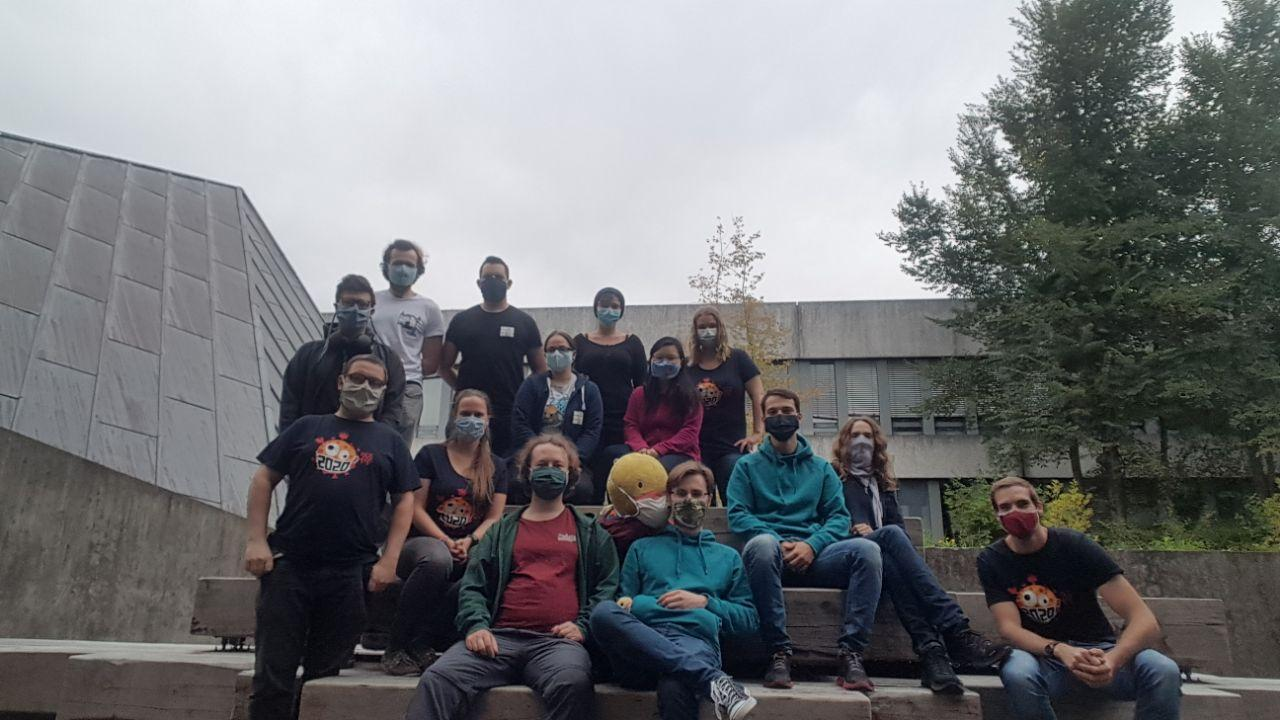
\includegraphics[width=.6\textwidth]{klausurtagung.jpg}
\end{frame}


\begin{frame}{Akkreditierungspool}
    \begin{itemize}
        \item Der studentische Akkreditierungspool
        \begin{itemize}
        	\item sorgt für die Einflussnahme von Studierenden in Akkreditierungsverfahren
        	\item entsendet Studierendenvertreter in den Akkreditierungsrat und in Agentur- und (extern besetzte) Hochschulgremien
        	\item vertritt studentische Interessen gegenüber Agenturen und anderen Stakeholdern
        \end{itemize}         
        \item Studierende werden vorher in Seminaren geschult. \\
          {\scriptsize\color{blue} Nächste Termine (digital \& analog): siehe Webseite \url{https://www.studentischer-pool.de}}
        \item Nächstes Poolvernetzungstreffen wohl hybrid {\color{blue} (November/Dezember)}
        \vspace{0.5cm}
        \item[$\rightarrow$] Bei Interesse: Besucht den Akkreditierungs-Workshop für Einsteiger
    \end{itemize}
\end{frame}


\section{TOPF}

\begin{frame}{Was ist der TOPF?}
  \begin{minipage}{.5\textwidth}
    \begin{itemize}
      \item 2 DECkEL \footnotemark[1]
      \begin{itemize}
        \item Sean Bonkwoski (Bonn)
        \item Timo Prinz (Berlin, TU)
      \end{itemize}
      \item Viele HENkeL\footnotemark[2]\footnotemark[3]
      \item Server
      \item ... und ganz viele Dienste
    \end{itemize}
  \end{minipage}
  \hfill
  \begin{minipage}{.48\textwidth}
    \begin{minipage}[c]{.5\textwidth}
      
\includegraphics[height=.4\textheight]{sean.jpg}
      \captionof*{figure}{Sean}
    \end{minipage}
    \begin{minipage}[c]{.48\textwidth}
      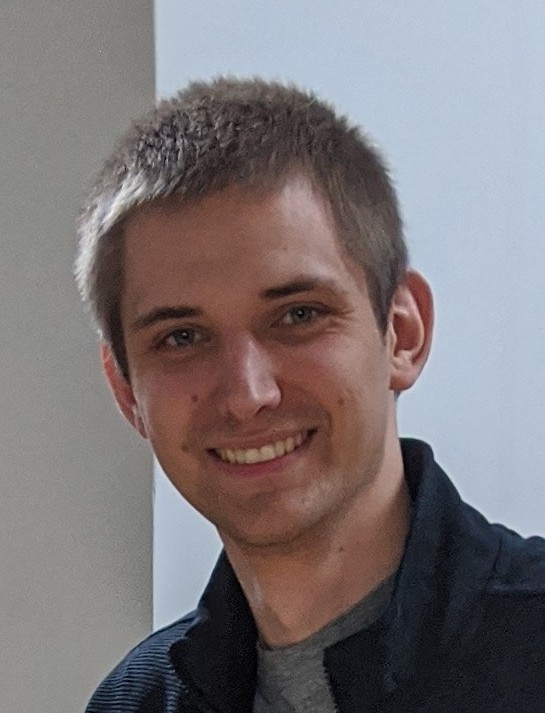
\includegraphics[height=.4\textheight]{timo.jpg}
      \captionof*{figure}{Timo}
    \end{minipage}
  \end{minipage}
  \footnotetext[1]{Dokumentations-, Einrichtungs- und Clusterfuckkoordinierende für EDV-Lösungen} 
  \footnotetext[2]{Helfende mit EDV- und Netzwerkkompetenzen für ergebnisorentierte Lösungen}
  \footnotetext[3]{Können gerne mehr werden ;-)}
\end{frame}

\section{KomGrem}

\begin{frame}\frametitle{KomGrem - Wer sind wir?}
 \begin{figure}
		\begin{subfigure}[t]{0.24\textwidth}
			
\includegraphics[width = \textwidth]{brunner.jpg}
			\caption*{Jacob Brunner (Augsburg)}
		\end{subfigure}
			\begin{subfigure}[t]{0.24\textwidth}
				
\includegraphics[width = \textwidth]{blaensdorf.jpg}
				\caption*{Sebastian Blänsdorf (Heidelberg)}
		\end{subfigure}
			\begin{subfigure}[t]{0.24\textwidth}
				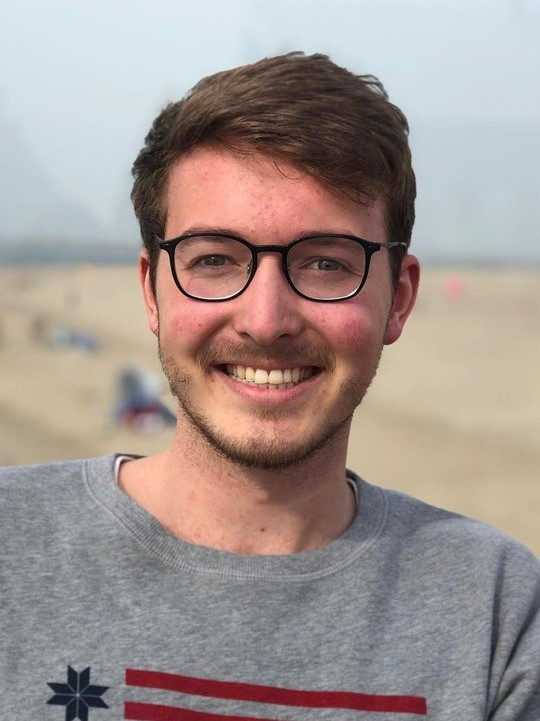
\includegraphics[width = \textwidth]{Nitschke.jpeg}
				\caption*{Jonah Nitschke (jDPG RG Dortmund)}
		\end{subfigure}
				\begin{subfigure}[t]{0.24\textwidth}
				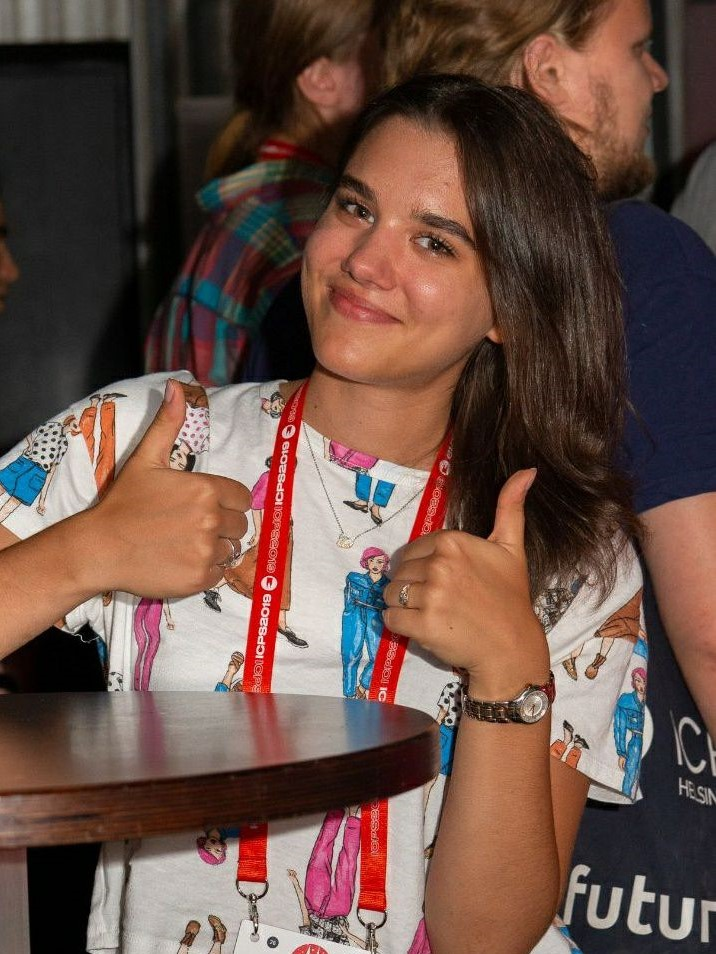
\includegraphics[width = \textwidth]{boushmelev.jpg}
				\caption*{Anastasia Boushmelev (jDPG RG Siegen)}
		\end{subfigure}
 \end{figure}
\end{frame}

\begin{frame}\frametitle{KomGrem - Was machen wir?}
	\begin{block}{Was wir machen}
		\begin{itemize}
			\item Koordinierung der Zusammenarbeit von jDPG und ZaPF
			\item Austausch über mögliche Kooperationen bei verschiedenen Themen (CHE, Nachhaltigkeit etc.)
			\item Teilnahme an der KFP (Konferenz der Fachbereiche Physik)
			\item Verbesserung der Vernetzung zwischen Fachschaften und jDPG Regionalgruppen
		\end{itemize}
	\end{block}
\end{frame}

\section{ZaPF e.V.}

\begin{frame}{Was tut der ZaPF e.V.?}
  \begin{block}{Aufgaben des e.V.}
    \begin{itemize}
      \item Strukturelle Unterstützung der ZaPF
      \item Infrastruktur
      \item Finanzielle Absicherung
      \item Rechtliche Absicherung
      \item Finanzierung für Gremien (z.B. Reisekosten)
      \item Unterstützung von Finanzschwachen Fachschaften
    \end{itemize}
  \end{block}
\end{frame}
  
\begin{frame}{Wer tut da was im ZaPF e.V.?}
  \begin{block}{Aktuelle Vorstände}
    \begin{minipage}{0.5\textwidth}
      \begin{figure}
      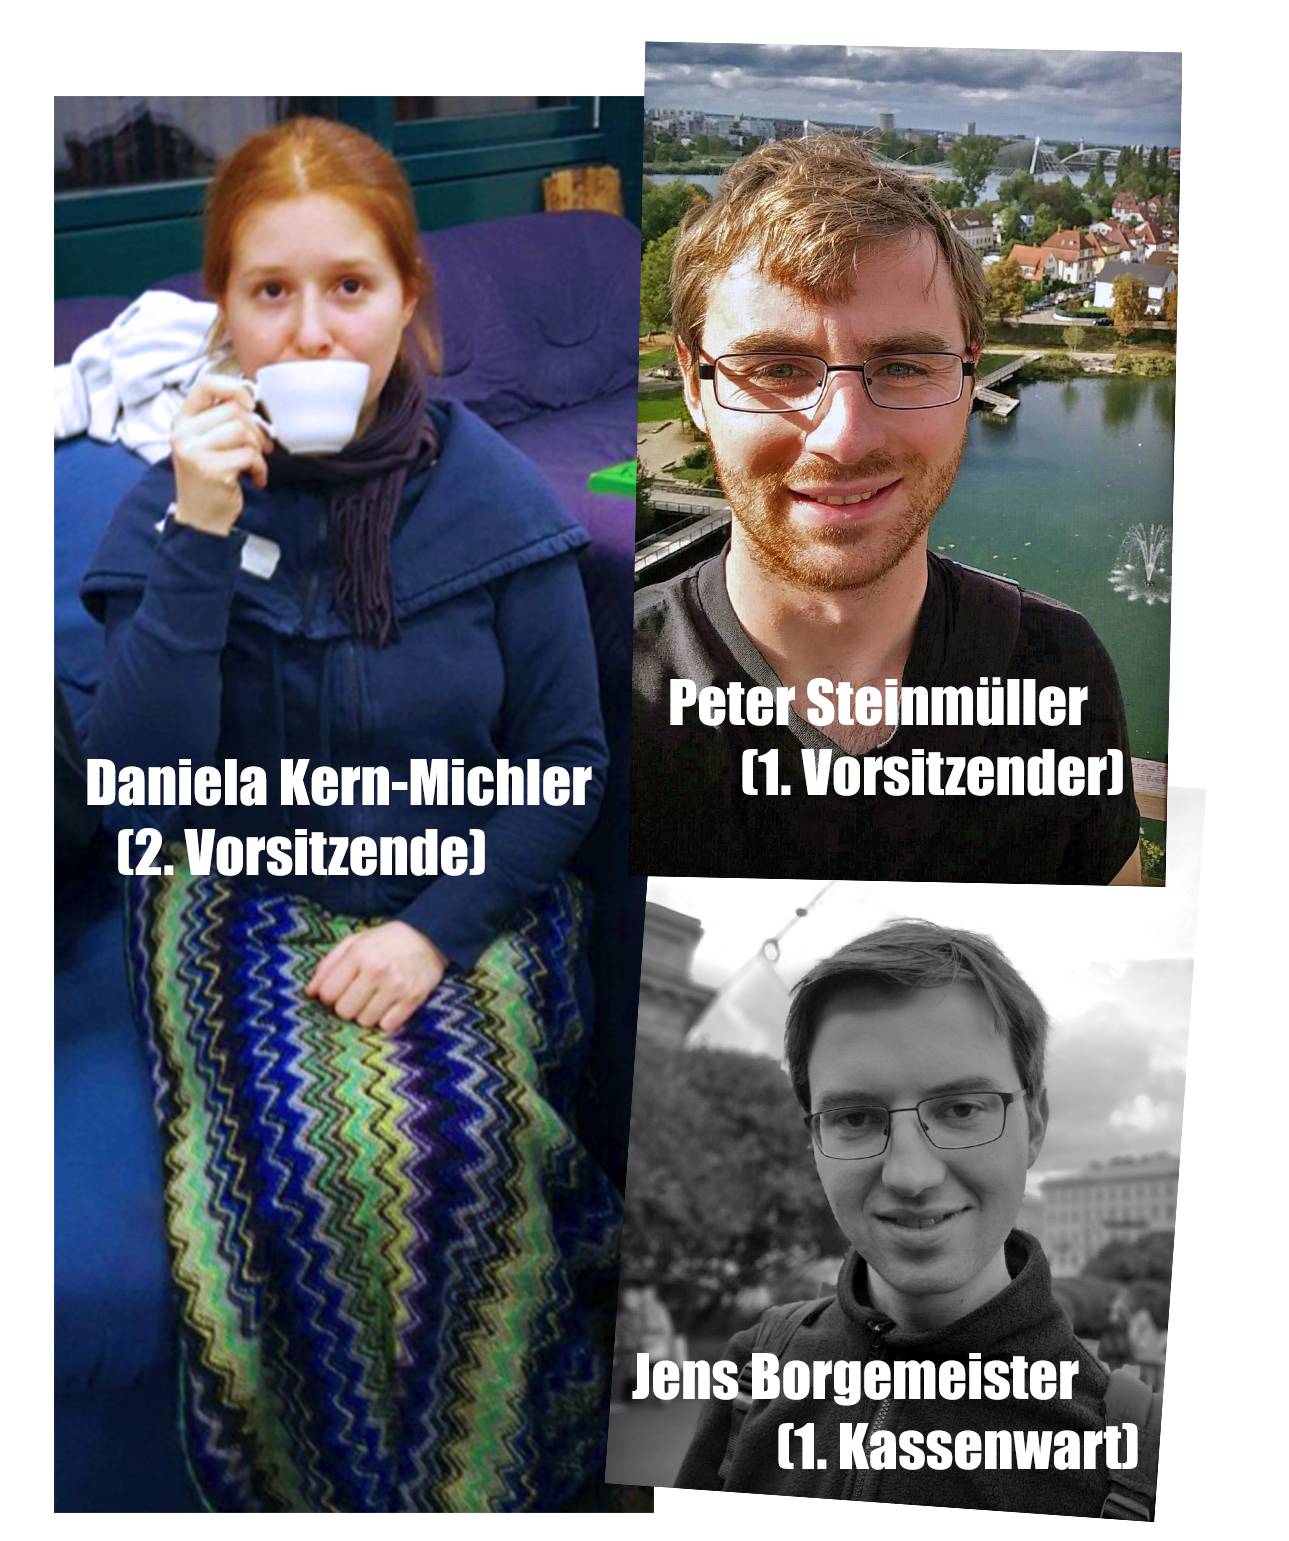
\includegraphics[height=.75\textheight]{ZapfeV.png}
      \end{figure}
    \end{minipage}
    \begin{minipage}{0.45\textwidth}
      \begin{itemize}
        \item Marcus Mikorski \mbox{(2. Kassenwart)}
        \item Fabian Freyer (IT)
        \item Lisa Dietrich (Finanzschwache Fachschaften)
        \item Marcel Nitsch (Bonn)
        \item Timo Rachel (Freiburg)
        \item Lena Wunderl (München)
        \item Richard Altenkirch (Rostock)
      \end{itemize}
    \end{minipage}
  \end{block}
\end{frame}
  
\begin{frame}{Was kann man tun im ZaPF e.V.?}
  \begin{block}{Fördermitglied werden}
    \begin{itemize}
    \item Fördermitglieder sind natürliche Personen (z.B. du) oder juristische (euer Fachschaft oder Verein)
    \item Ihr unterstützt den Verein mit Mitgliederbeiträgen
    \end{itemize}
  \end{block}
  \begin{block}{Mitglied werden}
    \begin{itemize}
    \item Normale Mitglieder entscheiden über die Tätigkeiten des Vereins
    \item Diese zahlen keinen Beitrag
    \end{itemize}
  \end{block}
\end{frame}
  
\begin{frame}{Mitgliederversammlung am 12.11. um 19 Uhr}
  \begin{block}{Tagesordnung}
    \begin{multicols}{2}
      \begin{enumerate}\small
        \item Feststellung der Tagesordnung
        \item Wahl des Protokollführers
        \item Wahl der Versammlungsleitung
        \item Feststellung der Beschlussfähigkeit
        \item Genehmigung der letzten Protokolle
        \item Bericht des Vorstands
        \item Bericht des Kassenprüfers
        \item Umgang mit Corona Situtation
        \item Sonstiges
      \end{enumerate}
    \end{multicols}
  \end{block}
  \begin{block}{Ort}
    Die MV findet Online statt. Der Link dazu wird in den kommenden Tage im ZaPF-Wiki (\url{https://zapf.wiki/WiSe20_MV_ZaPFeV}) veröffentlicht.
  \end{block}
\end{frame}

\begin{frame}{Mitgliederversammlung am 12.11. um 19 Uhr}
  \begin{block}{Corona Situation}
    Die MV wird rein informell sein.\\
    Personenwahlen sind (aktuell) nicht online möglich.\\
    Der Vorstand bleibt, entsprechend dem Corona-Gesetz, bis zur nächsten Wahl bestehen.\\[1.5em]
    Nach der ZaPF soll es eine MV für Neuwahlen geben, welche dann in Person stattfinden soll.
  \end{block}
\end{frame}

\begin{frame}{Kommende ZaPFen}
  \begin{itemize}
    % \vspace{05cm}
    \item Sommersemester 2021 in Rostock und Greifswald
    \item Wintersemester 2021 in Göttingen
    \item Sommersemester 2022 \textit{\color{blue}{bei euch?}}    
\end{itemize}
    \vspace{1cm}
    \begin{center}
      \huge \textbf{Tosenden Applaus für die ausrichtenden Orgas!}
    \end{center}
\end{frame}

\begin{frame}[plain]
  \begin{center}
    \Huge Habt ihr Fragen an uns?
    \end{center}
\end{frame}


\section{Wissenschaftskommunikation}

\end{document}
